\documentclass{lecture}

%\batchmode

\usepackage{multicol}
\setlength{\columnseprule}{0.4pt}

\usepackage{pdflscape}

\usepackage{math}
\usepackage{ncolor}
\setprimary{black}

\begin{document}
\begin{landscape}

\course{COMP3506}

\begin{multicols}{2}

    \heading{RAM Model}
    \begin{note}{Memory}
        Infinite sequence of cells, contains $w$ bits. Every cell has an address starting at 1
    \end{note}
    \vfill
    \begin{note}{CPU}
        32 registers of width $w$ bits.
        \subheading{Operations}
        Set value to register (constant or from other register). Take two integers from other registers and store the result of; $a+b$, $a-b$, $a\cdot b$, $a/b$. Take two registers and compare them; $a<b$ $a=b$, $a>b$. Read and write from memory.
        \subheading{Definitions}
        An algorithm is a set of atomic operations. It's cost is the number of atomic operations. A word is a sequence of $w$ bits
    \end{note}
    \vfill

    \heading{Definitions}
    \begin{note}{Worst-case}
        Worst-case cost of an algorithm is the longest possible running time of input size $n$
    \end{note}
    \vfill
    \begin{note}{Random}
        RANDOM(x, y) returns an integer between x and y chosen uniformly at random
    \end{note}
    \vfill
    \begin{note}{Data Structure}
        Data Structure describes how data is stored in memory.
    \end{note}
    \vfill
    \begin{note}{Dictionary Search}
        let $n$ be register 1, and $v$ be register 2\\
        register $left\rightarrow 1$, $right\rightarrow1$\\
        while $left\leq right$\\
        \indent register $mid\rightarrow(left+right)/2$\\
        \indent if the memory cell at address $mid=v$ then\\
        \indent\indent return yes\\
        \indent else if memory cell at address $mid>v$ then\\
        \indent\indent $right=mid-1$\\
        \indent else\\
        \indent\indent $left=mid+1$\\
        return no\\\\
        Worst-case time: $f_2(n)=2+6\log_2n$
    \end{note}
    \vfill

    \heading{Function Comparison}
    \begin{note}{Big-O}
        We say that $f(n)$ grows asymptotically no faster than $g(n)$ if there is a constant $c_1>0$ such that $f(n)\leq c_1\cdot g(n)$ and holds for all $n$ at least a constant $c_2$. This is denoted by $f(n)=O(g(n))$.\\
        $\lim_{n\rightarrow\infty}\frac{f(n)}{g(n)}=c$ for some constant $c$
        \subheading{Example}
        $1000\log_2n=O(n)$,\\$n\neq O(10000\log_2n)$\\
        $\log_{b_1}n=O(\log_{b_2}n)$ for any constants $b_1>1$ and $b_2>1$.
        Therefore $f(n)=2+6\log_2n$ can be represented; $f(n)=O(\log n)$
    \end{note}
    \vfill
    \begin{note}{Big-$\Omega$}
        If $g(n)=O(f(n))$, then $f(n)=\Omega(g(n))$ to indicate that $f(n)$ grows asymptotically no slower than $g(n)$. We say that $f(n)$ grows asymptotically no slower than $g(n)$ if $c_1>0$ such $f(n)\geq c_1\cdot g(n)$ for $n>c_2$; denoted by $f(n)=\Omega(g(n))$
    \end{note}
    \vfill
    \begin{note}{Big-$\Theta$}
        If $f(n)=O(g(n))$ and $f(n)=\Omega(g(n))$, then $f(n)=\Theta(g(n))$ to indicate that $f(n)$ grows asymptotically as fast as $g(n)$
    \end{note}

    \vspace{1em}\heading{Sort}
    \begin{note}{Merge Sort}
        Divide the array into two parts, sort the individual arrays then combine the arrays together. $f(n)=O(n\log n)$.\\
        This is the fastest sorting time possible (apart from $O(n\log\log n)$
    \end{note}
    \vfill
    \begin{note}{Counting Sort}
        A set S of n integers and every integer is in the range [1, U]. (all integers are distinct)\\
        \textbf{Step 1:} Let A be the array storing S. Create array B of length U. Set B to zero.\\
        \textbf{Step 2:} For $i\in [1,n]$; Set x to A[i], Set B[x] = 1\\
        \textbf{Step 3:} Clear A, For $x\in[1,U]$; If B[x] = 0 continue, otherwise append x to A
        \subheading{Analysis}
        Step 1 and 3 take O(U) time, while Step 2 O(n) time. Therefore running time is O(n + U) = O(U).
    \end{note}
    \vfill

    \heading{Data}
    \begin{note}{LinkedList}
        Every node stores pointers to its succeeding and preceding nodes (if they exist). The first node is called the head and last called the tail. The space required for a linkedlist is $O(n)$ memory cells. Starting at the head node, the time to enumerate over all the integers is $O(n)$. Time for assertion and deletion is equal to $O(1)$
    \end{note}
    \vfill
    \begin{note}{Stack}
        The stack has two operations; Push (Inserts a new element into the stack), Pop (Removes the most recently inserted element from the stack and returns it. Since a stack is just a linkedlist, push and pop use $O(1)$ time.
    \end{note}
    \vfill
    \begin{note}{Queue}
		The queue has two operations; En-queue (Inserts a new element into the queue), De-queue (Removes the least recently used element from the queue and returns it). Since a queue is just a linkedlist, push and pop use $O(1)$ time.<Paste>
    \end{note}
    \vfill

    \heading{Dynamic Arrays}
    \begin{note}{Naive Algorithm}
        \textbf{insert(e):} Increase n by 1, initial an array A' of length n, copy all n-1 of A to A', Set A'[n]=e, Destroy A.\\
        This takes $O(n^2)$ time to do $n$ insertions.
    \end{note}
    \vfill
    \begin{note}{A Better Algorithm}
        \textbf{insert(e):} Append e to A and increase n by 1. If A is full; Create A' of length 2n, Copy A to A', Destroy A and replace with A'\\
        This takes $O(n)$ time to do $n$ insertions.
    \end{note}
    \vfill

    \heading{Hashing}
    \begin{note}{}
        The main idea of hashing is to divide the dataset S into a number m of disjoint subsets such that only one subset needs to be searched to answer any query.
    \end{note}
    \vfill
    \begin{note}{Pre-processing}
        Create an array of linkedlist($L$) from 1 to $m$ and an array $H$ of length $m$. Store the heads of $L$ in $H$, for all $x\in S$; calculate hash value ($h(x)$), insert $x$ into $L_{h(x)}$. We will always choose $m=O(n)$, so $O(n+m)=O(n)$
    \end{note}
    \vfill
    \begin{note}{Querying}
        Query with value $v$, calculate the hash value $h(v)$, Look for $v$ in $L_h(v)$. Query time: $O(\mid L_{h(v)}\mid)$
    \end{note}
    \vfill
    \begin{note}{Hash Function}
        Pick a prime $p$; $p\geq m$, $p\geq$ any integer $k$. Choose $\alpha$ and $\beta$ uniformly random from $1,\ldots,p-1$. Therefore: $h(k)=1+(((\alpha k+\beta)mod\ p)mod\ m)$
    \end{note}
    \vfill
    \begin{note}{Any Possible Integer}
        The possible integers is finite under the RAM Model. Max: $2^w-1$. Therefore $p$ exists between $[2^w,w^{w+1}]$.
    \end{note}
    \vfill
    \begin{note}{Timing}
        Space: $O(n)$, Preprocessing time: $O(n)$, Query time: $O(1)$ in expectation
    \end{note}
    \vfill

    \heading{Week 3 -- Extra}
    \begin{note}{}
        When using `Direction 1: Constant Finding' setting $c_1$, always set it to match the coefficent on the LHS so that you can cancel.\\
        When trying to get a contradiction, try and isolate an $x \cdot c_1$ on the RHS, where $x \in Z$, such that an expression that contains $n$ is $\leq x \cdot c_1$\\
        Make judicious use of the $max$ function when adding functions together
        If $f_1(n) + f_2(n) \leq c_1 \cdot g_1(n) +c'_1 \cdot g_2(n) \leqslant max\{c_1 , c'_1 \} \cdot (g_1(n) + g_2(n))$, for all $n \geqslant max\{c_2, c'_2\}$.\\
    \end{note}
    \vfill

    \heading{The Master Theorem}
    \begin{note}{Theorem 1}
        $n+\frac{n}{c}+\frac{n}{c^2}+\ldots+\frac{n}{c^h}=O(n)$
    \end{note}
    \vfill
    \begin{note}{Theorem 2}
        Let $f(n)$ be a function that returns a positive value for every integer $n>0$. We know:
        \begin{align*}
            f(1) & \leqslant c_1\\
            f(n) & \leqslant \alpha \cdot f(\lceil n / \beta \rceil) + c_2 \cdot n^{\gamma} \text{ for } n \geqslant 2
        \end{align*}
        where $\alpha, \beta, \gamma, c_1$ and $c_2$ are positive constants. Then:
        \begin{itemize}[nolistsep]
            \item If $log_{b} \alpha < \gamma$ then $f(n) = O(n^\gamma)$
            \item If $log_{b} \alpha = \gamma$ then $f(n) = O(n^\gamma \cdot log(n))$
            \item If $log_{b} \alpha > \gamma$ then $f(n) = O(n^{log_\beta(a)})$
        \end{itemize}
    \end{note}
    \vfill

    \heading{Hierarchy}
    \begin{note}{}
        $$O(1) \leqslant O(log(n)) \leqslant O(n^c)$$ 
        $$\leqslant O(n) \leqslant O(n^2)$$ 
        $$\leqslant O(n^c) \leqslant O(c^n)$$
    \end{note}
    \vfill

    \heading{Trees}
    \begin{note}{Undirected Graphs}
        An undirected graph is a pair of (V, E) where:
        \begin{itemize}[nolistsep]
            \item V is a set of elements, each of which called a node.
            \item E is a set of pairs (u, v) such that:
                \begin{itemize}[nolistsep]
                    \item u and v are distinct nodes;
                    \item If (u, v) is in E, then (v, u) is also in E -- we say that there is an edge between u and v.
                \end{itemize}
        \end{itemize}
        A node may also be called a vertex. We will refer to V as the vertex set or the node set of the graph, and E the edge set.
    \end{note}
    \vfill
    \begin{note}{Paths and Cycles}
        Let G = (V, E) be an undirected graph. A path in G is a sequence of nodes $(v_1, v_2, \ldots, v_k)$ such that
        \begin{itemize}[nolistsep]
            \item For every $i\in [1, k-1]$, there is an edge between $v_i$ and $v_{i+1}$.
        \end{itemize}
        A cycle in G is a path $(v_1, v_2, \ldots, v_k)$ such that; $k\geq 4$, $v_1 = v_k$, $v_1, v_2, \ldots, v_{k-1}$ are distinct
    \end{note}
    \vfill
    \begin{note}{Connected Graphs}
        An undirected graph G = (V, E) is connected if, for any two distinct vertices u and v, G has a path from u to v.
    \end{note}
    \vfill
    \begin{note}{Trees}
        A tree is a connected undirected graph contains no cycles.
    \end{note}
    \vfill
    \begin{note}{Rooting a Tree}
        Given any tree T and an arbitrary node r, we can allocate a level to each node as follows:
        \begin{itemize}[nolistsep]
            \item r is the root of T -- this is level 0 of the tree.
            \item All the nodes that are 1 edge away from r constitute level 1 of the tree.
            \item All the nodes that are 2 edges away from r constitute level 2 of the tree.
            \item And so on.
        \end{itemize}
        The number of levels is called the height of the tree. We say that T has been rooted once a root has been designated.
    \end{note}
    \vfill
    \begin{note}{Ancestors and Descendants}
        Let u and v be two nodes in T. u is an ancestor of v is one of the following holds: u = v, u is the parent of v, u is the parent of an ancestor of v.\\
        Accordingly, we say that v is a descendant of u. In particular, if $u\neq v$, we say that u is a proper ancestor of v, and likewise, v is a proper descendant of u.\\
        \begin{multicols}{2}
        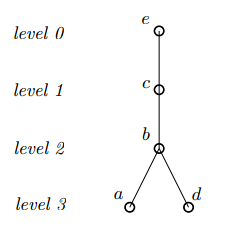
\includegraphics[width=\linewidth]{ancestor}
        Node b is an ancestor of b, a and d.\\
        Node c is an ancestor of c, b, a and d.\\
        Node c is a proper ancestor of b, a, d.
        \end{multicols}
    \end{note}
    \vfill
    \begin{note}{Subtrees}
        The subtree of u is the part of T that is ``at or below'' u.
    \end{note}
    \vfill
    \begin{note}{Internal and Leaf Nodes}
        In a rooted tree, a node is a leaf node if it has no children; otherwise, it is an internal node.
    \end{note}
    \vfill
    \begin{note}{k-Ary and Binary}
        A k-Ary tree is a rooted tree where every internal node has at most k child nodes. A 2-ary tree is called a binary tree.
    \end{note}
    \begin{note}{Full Level}
        Consider a binary tree with height $h$. Its Level $l (0\leq l \leq h-1)$ is full if it contains $2^l$ nodes.
    \end{note}
    \vfill
    \begin{note}{Complete Binary Tree}
        A binary tree of height $h$ is complete if:
        \begin{itemize}[nolistsep]
            \item Levels 0, 1, \ldots, h-2 are all full
            \item At Level h-1, the leaf nodes are ``as far left as possible''.\\
                This means that if you were to add a leaf node v at Level h-1, v would need to be on the right of all the existing leaf nodes.
        \end{itemize}
    \end{note}
    \vfill

    \heading{Priority Queue}
    \begin{note}{}
        A priority queue stores a set S of n integers and supports the following operations:
        \begin{itemize}[nolistsep]
            \item Insert(e): Adds a new integer to S.
            \item Delete-min: Removes the smallest integer in S, and returns it.
        \end{itemize}
    \end{note}
    \vfill
    \begin{note}{}
        Next we will implement a priority queue using a data structure called the binary heap to achieve the following guarantees:
        \begin{itemize}[nolistsep]
            \item O(n) space consumption
            \item O(log n) insertion time
            \item O(log n) delete-min time
        \end{itemize}
    \end{note}
    \vfill

    \heading{Binary Heap}
    \begin{note}{}
        Let S be a set of n integers. A binary heap on S is a binary tree T satisfying:
        \begin{itemize}[nolistsep]
            \item T is complete
            \item Every node u in T corresponds to a distinct integer in S -- the integer is called the key of u (and is stored at u).
            \item If u is an internal node, the key of u is smaller than those of its child noeds.
        \end{itemize}
        Two possible binary heaps on S = \{93, 39, 1, 26, 8, 23, 79, 54\}:
        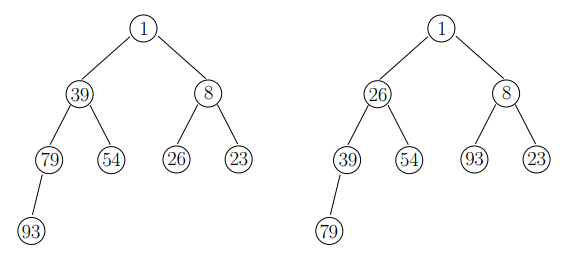
\includegraphics[width=\linewidth]{binaryheap}
        The smallest integer of S must be the key of the root.
    \end{note}
    \vfill
    \begin{note}{Insertion}
        We preform insert(e) on a binary heap T as follows:
        \begin{enumerate}[nolistsep]
            \item Create a leaf node z with key e, while ensuring that T is a complete binary tree -- notice that there is only one place where z can be added.
            \item Set $u\rightarrow z$.
            \item If u is the root, return.
            \item If the key of $u >$ the key of its parent p, return.
            \item Otherwise, swap the keys of u and p. Set $u\rightarrow p$, and repeat from Step 3.
        \end{enumerate}
    \end{note}
    \vfill
    \begin{note}{Delete-Min}
        We perform a delete-min on a binary heap T as follows:
        \begin{enumerate}[nolistsep]
            \item Report the key of the root.
            \item Identify the rightmost leaf z at the bottom level of T.
            \item Delete z, and store the key of z at the root.
            \item Set $u\rightarrow$ the root.
            \item If $u$ is a leaf, return.
            \item If the key of $u <$ the keys of the children of u, return.
            \item Otherwise, let v be the child of u with a smaller key. Swap the keys of u and v. Set $u\rightarrow v$, and repeat from Step 5.
        \end{enumerate}
    \end{note}

\end{multicols}

\end{landscape}
\end{document}
